% Source-relative PDF page 1, Q9 (printed page 302).
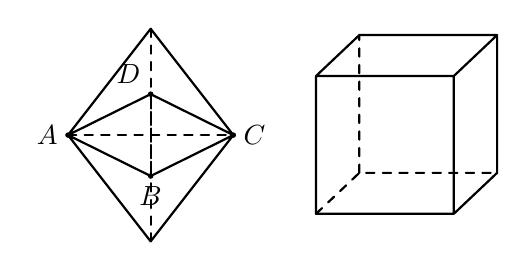
\begin{tikzpicture}[line cap=round,line join=round,thick]
  % Two congruent square pyramids sharing the square ABCD.
  \coordinate (A) at (0,1.0); \coordinate (B) at (1.05,0.48);
  \coordinate (C) at (2.1,1.0); \coordinate (D) at (1.05,1.52);
  \coordinate (T) at (1.05,2.35); \coordinate (S) at (1.05,-0.35);
  \draw[dashed] (A)--(C) (T)--(B) (S)--(D);
  \draw (A)--(D)--(C) (A)--(B)--(C) (T)--(A) (T)--(C) (S)--(A) (S)--(C);
  \fill (A) circle (1pt) node[left] {$A$};
  \fill (B) circle (1pt) node[below] {$B$};
  \fill (C) circle (1pt) node[right] {$C$};
  \fill (D) circle (1pt) node[above left] {$D$};
  % Unit cube; hidden rear-left edges are dashed.
  \begin{scope}[xshift=3.15cm]
    \coordinate (a) at (0,0); \coordinate (b) at (1.75,0);
    \coordinate (c) at (1.75,1.75); \coordinate (d) at (0,1.75);
    \coordinate (e) at (0.55,0.52); \coordinate (f) at (2.3,0.52);
    \coordinate (g) at (2.3,2.27); \coordinate (h) at (0.55,2.27);
    \draw (a)--(b)--(c)--(d)--cycle (b)--(f)--(g)--(c) (d)--(h)--(g);
    \draw[dashed] (a)--(e)--(f) (e)--(h);
  \end{scope}
\end{tikzpicture}
